% Informe final (hito 3) - formato IEEE de conferencia, doble columna. Compilar en Overleaf con pdfLaTeX + BibTeX.
% Todas las cifras vienen de cifras.tex y tablas/*.tex, generados por: python -m src.make_report_tables
% (a partir de experiments/). No escriba números a mano: vuelva a generar esos archivos.
\documentclass[conference]{IEEEtran}
\IEEEoverridecommandlockouts
\usepackage[utf8]{inputenc}
\usepackage[T1]{fontenc}
\usepackage[spanish,es-nodecimaldot,es-noshorthands]{babel}
\usepackage{amsmath,amssymb}
\usepackage{graphicx}
\usepackage{booktabs}
\usepackage{xcolor}
\usepackage{url}
\usepackage{tikz}
\usetikzlibrary{positioning,arrows.meta,fit}
\usepackage[hidelinks]{hyperref}
\newcommand{\pend}[1]{\textcolor{red}{\textbf{[#1]}}}
% GENERADO por python -m src.make_report_tables. No editar a mano.
\newcommand{\CifraNRaw}{8.066}
\newcommand{\CifraNDup}{573}
\newcommand{\CifraN}{7.493}
\newcommand{\CifraNFatal}{569}
\newcommand{\CifraNHeridos}{6.924}
\newcommand{\CifraPctFatal}{7,6\,\%}
\newcommand{\CifraCoordFuera}{26}
\newcommand{\CifraIncoherentes}{282}
\newcommand{\CifraMuertosDosMilVeinticinco}{361}
\newcommand{\CifraTipoViaDesconocido}{50,3\,\%}
\newcommand{\CifraObjetoSinDato}{94,0\,\%}
\newcommand{\CifraChoqueSinDato}{24,9\,\%}
\newcommand{\CifraNBarrios}{220}
\newcommand{\CifraNHipotesis}{88}
\newcommand{\CifraNTrain}{4.850}
\newcommand{\CifraFatTrain}{341}
\newcommand{\CifraPctTrain}{7,03\,\%}
\newcommand{\CifraNVal}{1.253}
\newcommand{\CifraFatVal}{113}
\newcommand{\CifraPctVal}{9,02\,\%}
\newcommand{\CifraNTest}{1.390}
\newcommand{\CifraFatTest}{115}
\newcommand{\CifraPctTest}{8,27\,\%}
\newcommand{\CifraTasaGlobal}{7,4\,\%}
\newcommand{\CifraTasaMadrugada}{13,5\,\%}
\newcommand{\CifraTasaManana}{5,3\,\%}
\newcommand{\CifraTasaTarde}{5,8\,\%}
\newcommand{\CifraTasaNoche}{8,9\,\%}
\newcommand{\CifraTasaAtropello}{11,9\,\%}
\newcommand{\CifraTasaChoque}{5,8\,\%}
\newcommand{\CifraTasaCaida}{16,2\,\%}
\newcommand{\CifraTasaObjetoFijo}{24,0\,\%}
\newcommand{\CifraTasaVehiculo}{5,3\,\%}
\newcommand{\CifraTasaDosMilVeinte}{5,9\,\%}
\newcommand{\CifraTasaDosMilVeinticuatro}{9,0\,\%}
\newcommand{\CifraBasePR}{0,220}
\newcommand{\CifraBaseROC}{0,666}
\newcommand{\CifraBasePrec}{0,136}
\newcommand{\CifraBaseRec}{0,637}
\newcommand{\CifraBaseAzar}{0,090}
\newcommand{\CifraBaseAcc}{0,910}
\newcommand{\CifraBasePRAntes}{0,229}
\newcommand{\CifraUmbral}{0,1085}
\newcommand{\CifraValPR}{0,224}
\newcommand{\CifraValPRsd}{0,004}
\newcommand{\CifraValROC}{0,699}
\newcommand{\CifraValROCsd}{0,006}
\newcommand{\CifraValPrec}{0,179}
\newcommand{\CifraValRec}{0,602}
\newcommand{\CifraValAlerta}{30,2\,\%}
\newcommand{\CifraValPRMovil}{0,180}
\newcommand{\CifraValDifPR}{0,004}
\newcommand{\CifraValPrecMedia}{0,166}
\newcommand{\CifraRFHojas}{5}
\newcommand{\CifraRFMaxFeat}{sqrt}
\newcommand{\CifraDuracionBusqueda}{206}
\newcommand{\CifraNConfig}{33}
\newcommand{\CifraAblContexto}{0,176}
\newcommand{\CifraAblReporte}{0,224}
\newcommand{\CifraAblHipotesis}{0,273}
\newcommand{\CifraAblHipotesisROC}{0,745}
\newcommand{\CifraAblHipotesisPrec}{0,210}
\newcommand{\CifraValPeorSubgrupo}{Mañana}
\newcommand{\CifraValPeorRecall}{0,210}
\newcommand{\CifraTestPR}{0,223}
\newcommand{\CifraTestPRic}{[0,166; 0,299]}
\newcommand{\CifraTestROC}{0,712}
\newcommand{\CifraTestROCic}{[0,667; 0,761]}
\newcommand{\CifraTestPrec}{0,157}
\newcommand{\CifraTestPrecic}{[0,119; 0,198]}
\newcommand{\CifraTestRec}{0,470}
\newcommand{\CifraTestRecic}{[0,381; 0,560]}
\newcommand{\CifraTestAlerta}{24,7\,\%}
\newcommand{\CifraTestFN}{61}
\newcommand{\CifraTestTP}{54}
\newcommand{\CifraTestFP}{289}
\newcommand{\CifraTestTN}{986}
\newcommand{\CifraTestBasePR}{0,154}
\newcommand{\CifraTestBasePRic}{[0,118; 0,203]}
\newcommand{\CifraTestBaseROC}{0,689}
\newcommand{\CifraTestDifPR}{0,069}
\newcommand{\CifraCommitFinal}{e58aacf}
\newcommand{\CifraTestTardeRec}{0,118}
\newcommand{\CifraTestTardeic}{[0,000; 0,308]}
\newcommand{\CifraTestTardeFat}{17}
\newcommand{\CifraTestBrechaTarde}{0,352}
\newcommand{\CifraTestBrechaTardeBase}{0,151}
\newcommand{\CifraTasaLocUno}{6,7\,\%}
\newcommand{\CifraTestRecLocUno}{0,605}
\newcommand{\CifraTestRecLocUnoic}{[0,45; 0,76]}
\newcommand{\CifraTasaLocDos}{8,5\,\%}
\newcommand{\CifraTestRecLocDos}{0,351}
\newcommand{\CifraTestRecLocDosic}{[0,20; 0,51]}
\newcommand{\CifraTasaLocTres}{7,7\,\%}
\newcommand{\CifraTestRecLocTres}{0,429}
\newcommand{\CifraTestRecLocTresic}{[0,27; 0,58]}
\newcommand{\CifraTestRecMadrugada}{0,583}
\newcommand{\CifraTestRecManana}{0,391}
\newcommand{\CifraTestRecNoche}{0,564}
\newcommand{\CifraMamonalAlerta}{47,5\,\%}
\newcommand{\CifraMamonalReal}{11,5\,\%}
\newcommand{\CifraMamonalVeces}{1,9}
\newcommand{\CifraNFN}{61}
\newcommand{\CifraNFP}{289}
\newcommand{\CifraFNChoqueVeh}{47}
\newcommand{\CifraFPAtropello}{144}
\newcommand{\CifraAlertaVal}{30,2\,\%}
\newcommand{\CifraAlertaTest}{24,7\,\%}
\newcommand{\CifraProbaVal}{0,089}
\newcommand{\CifraProbaTest}{0,081}
\newcommand{\CifraAtropelloVal}{13,7\,\%}
\newcommand{\CifraAtropelloTest}{9,5\,\%}
\newcommand{\CifraTardeVal}{8,9\,\%}
\newcommand{\CifraTardeTest}{4,1\,\%}
\newcommand{\CifraImpUno}{choque\_con}
\newcommand{\CifraImpUnoVal}{0,046}
\newcommand{\CifraImpDos}{lat}
\newcommand{\CifraImpDosVal}{0,025}
\newcommand{\CifraImpTres}{hora}
\newcommand{\CifraImpTresVal}{0,019}


\begin{document}

\title{¿Será fatal? Estimación de la gravedad de siniestros viales con víctimas en Cartagena a partir del informe inicial}

\author{
\IEEEauthorblockN{Juan Diego Rosales}
\IEEEauthorblockA{\pend{COMPLETAR POR EL EQUIPO: programa, universidad, ciudad}}
\and
\IEEEauthorblockN{Carolina Velasco Yanez}
\IEEEauthorblockA{\pend{COMPLETAR POR EL EQUIPO: programa, universidad, ciudad}}
}

\maketitle

% =====================================================================================================================
\begin{abstract}
Con los datos abiertos del Departamento Administrativo de Tránsito y Transporte (DATT) de Cartagena (2020--2025,
\CifraN{} siniestros con víctimas, \CifraPctFatal{} fatales) estudiamos si un modelo de aprendizaje supervisado puede estimar, solo
con el informe inicial (cuándo, dónde, clase de accidente y con qué chocó), si un siniestro será fatal. Comparamos una regresión
logística de referencia con una regresión logística ajustada, un \emph{random forest} y \emph{gradient boosting} de histogramas,
con partición temporal, validación de origen móvil, cinco semillas, ablación de variables y criterios de éxito declarados antes de
entrenar. El \emph{random forest} elegido obtuvo en la prueba de 2025, evaluada una sola vez, un PR-AUC de \CifraTestPR{}
\CifraTestPRic{} frente a \CifraTestBasePR{} de la línea base y un ROC-AUC de \CifraTestROC{}; sin embargo, con el umbral fijado
en validación su precisión fue \CifraTestPrec{} y su recall \CifraTestRec{}, y su recall en la franja de la tarde fue \CifraTestTardeRec{}.
Cumple solo uno de los cuatro criterios. Concluimos que el informe inicial contiene señal real pero insuficiente para una
herramienta operativa, y documentamos la deriva temporal, los errores dominantes y los riesgos de su uso.
\end{abstract}

\begin{IEEEkeywords}
siniestralidad vial, gravedad, aprendizaje supervisado, random forest, datos desbalanceados, IA responsable
\end{IEEEkeywords}

% =====================================================================================================================
\section{Introducción}
Los siniestros de tránsito causan cerca de 1,19 millones de muertes al año en el mundo \cite{who2023road}. En Cartagena, según cifras
del DATT publicadas en agosto de 2026, en lo corrido del año se registraron 1.134 siniestros y 95 fallecidos, 86 de ellos asociados a
motocicletas \cite{eluniversal2026motos}. Cuando se reporta un siniestro con víctimas, la información disponible es escasa: la
hora, el lugar, la clase de accidente y contra qué chocó. Si con esos datos se pudiera anticipar qué casos tienen más probabilidad
de terminar en muerte, el centro que coordina la respuesta (usuario objetivo: personal de despacho de emergencias y del DATT
\pend{CONFIRMAR usuario con el equipo}) podría priorizar la atención y el análisis posterior.

\textbf{Pregunta.} Dado un siniestro vial \emph{con víctimas} en Cartagena, ¿puede un modelo estimar con el informe inicial si será
fatal, mejor que una línea base, y con qué diferencias por franja horaria y localidad?

Las contribuciones son: (i) un pipeline reproducible sobre datos abiertos con corrección documentada de problemas de calidad;
(ii) una comparación de tres familias de modelos con protocolo temporal y criterios predeclarados; (iii) un análisis de errores,
de deriva temporal y de equidad por subgrupos medido en una prueba evaluada una sola vez; y (iv) un prototipo de apoyo.

% =====================================================================================================================
\section{Trabajo relacionado}
La predicción de la gravedad de siniestros tiene una larga tradición en modelos estadísticos (logit multinomial, probit ordenado,
modelos con heterogeneidad no observada), revisada por Mannering y Bhat \cite{mannering2014analytic}, quienes advierten que muchas
variables determinantes de la gravedad no se observan en los registros policiales. Iranitalab y Khattak \cite{iranitalab2017comparison}
compararon el logit multinomial con vecinos más cercanos, máquinas de soporte vectorial y \emph{random forests} para predecir la
gravedad en choques de dos vehículos en Nebraska, y propusieron evaluar los métodos según el costo de los errores.

En los métodos, los \emph{random forests} \cite{breiman2001rf} combinan árboles entrenados sobre remuestreos con selección aleatoria
de variables, lo que reduce la varianza y tolera interacciones no lineales. El \emph{gradient boosting} con histogramas, popularizado
por LightGBM \cite{ke2017lightgbm} e implementado en scikit-learn \cite{pedregosa2011sklearn}, ajusta árboles secuencialmente sobre
el gradiente de la pérdida y maneja variables categóricas de forma nativa. Russell y Norvig \cite{russell2020aima} enmarcan ambos
como aprendizaje supervisado con conjuntos de modelos y discuten la selección de modelos con datos de validación separados.

Sobre la evaluación, Saito y Rehmsmeier \cite{saito2015pr} muestran que con clases desbalanceadas la curva precisión--\emph{recall}
es más informativa que la ROC, lo que motiva nuestra métrica primaria. Kaufman et al.\ \cite{kaufman2012leakage} formalizan la
fuga de datos, que aquí aparece porque las columnas de conteo de víctimas definen la etiqueta. Tashman \cite{tashman2000outofsample}
recomienda la evaluación de origen móvil para datos ordenados en el tiempo, que usamos para ajustar hiperparámetros.

A diferencia de esos trabajos, nuestro problema restringe las variables a las del informe inicial, usa datos abiertos de una ciudad
colombiana y reporta explícitamente un resultado que no alcanza los criterios fijados de antemano.

% =====================================================================================================================
\section{Formulación}
\subsection{Agente y entorno (PEAS)}
\begin{table}[t]
\caption{Descripción PEAS del agente}\label{tab:peas}
\centering\small
\begin{tabular}{@{}p{0.2\columnwidth}p{0.72\columnwidth}@{}}
\toprule
Rendimiento & PR-AUC y F1 de la clase fatal; precisión con \emph{recall} $\geq 0{,}60$; \emph{recall} por franja y localidad. \\
Entorno & Flujo de siniestros con víctimas reportados al DATT en Cartagena. \\
Actuadores & Probabilidad estimada de fatalidad y alerta (pantalla del prototipo). \\
Sensores & Campos del informe inicial: fecha, hora, barrio, localidad, coordenadas, tipo de vía, clase de accidente, choque con, objeto fijo. \\
\bottomrule
\end{tabular}
\end{table}
La Tabla~\ref{tab:peas} resume el agente. El entorno es \emph{parcialmente observable} (no se conocen el vehículo, la velocidad
ni la víctima), \emph{estocástico}, \emph{episódico} (cada siniestro se evalúa de forma independiente), \emph{estático} durante la
decisión, de agente único y con percepciones mixtas, discretas y continuas \cite{russell2020aima}.

\subsection{Tarea formal}
Sea $x\in\mathcal{X}$ el vector de variables del informe (conjunto \texttt{reporte}: hora, mes, día, fin de semana, noche, latitud,
longitud, franja, barrio, localidad, tipo de vía, clase de accidente, choque con y objeto fijo) y $y\in\{0,1\}$ la etiqueta, con
$y=1$ si la gravedad registrada es «Con muertos» y $y=0$ si es «Con heridos». Con
$D_{\text{ent}}=\{(x_i,y_i): \text{año}_i\leq 2023\}$ se aprende $f:\mathcal{X}\to[0,1]$ que aproxima $P(y=1\mid x)$. La decisión
es $\hat y=\mathbb{1}[f(x)\geq\tau]$, con
$\tau=\max\{t: \text{recall}_{2024}(t)\geq 0{,}60\}$ elegido en validación (2024). La prueba (2025) se usa una sola vez.
Las variables \texttt{muertos}, \texttt{heridos} y \texttt{gravedad} definen $y$ y están excluidas de $x$ (fuga de datos
\cite{kaufman2012leakage}); cada script lo comprueba con una aserción.

% =====================================================================================================================
\section{Datos}
\textbf{Origen y licencia.} Conjunto «Accidentes de tránsito ocurridos en la ciudad de Cartagena de Indias», 2020--2025, publicado
por el DATT con licencia CC-BY \cite{datt2026dataset}. No contiene nombres ni documentos de identidad. El archivo descargado
tiene \CifraNRaw{} filas y 25 columnas; su SHA-256 queda registrado para verificar la reproducción.

\textbf{Preprocesamiento.} (1) Se eliminaron \CifraNDup{} filas con código IPAT repetido, conservando la de mayor gravedad.
(2) El archivo solo contiene siniestros con víctimas: \CifraNHeridos{} «Con heridos» y \CifraNFatal{} «Con muertos»
(\CifraPctFatal{}); el modelo, por tanto, no decide si hay víctimas. (3) Se derivaron hora, franja, mes, día y fin de semana;
\CifraCoordFuera{} coordenadas fuera de Cartagena se trataron como faltantes. (4) Al explorar los datos, antes de entrenar los
modelos propuestos, detectamos dos errores de codificación: el vacío de las columnas de vía viene como «0», lo que hacía constante
la variable \texttt{tipo\_via}, y la forma de registrar «sin dato» en \texttt{choque\_con} y \texttt{objeto\_fijo} cambia por año,
lo que permitía inferir el año del registro. Se corrigieron y la línea base se volvió a ejecutar (PR-AUC \CifraBasePRAntes{}
$\to$ \CifraBasePR{}); los umbrales de éxito no cambiaron. Tras la corrección, \texttt{tipo\_via} es desconocido en el
\CifraTipoViaDesconocido{} de los casos y \texttt{objeto\_fijo} no tiene dato en el \CifraObjetoSinDato{}.

\textbf{Calidad de la etiqueta.} En 2025 la columna \texttt{muertos} contradice a \texttt{gravedad} en \CifraIncoherentes{} filas
(ninguna entre 2020 y 2024) e implicaría \CifraMuertosDosMilVeinticinco{} siniestros mortales, incompatible con las cifras oficiales.
La etiqueta se toma de \texttt{gravedad} y \texttt{muertos} solo se audita.

\textbf{Partición temporal.} Entrenamiento 2020--2023 ($n=\CifraNTrain$, \CifraPctTrain{} fatales), validación 2024
($n=\CifraNVal$, \CifraPctVal{}) y prueba 2025 ($n=\CifraNTest$, \CifraPctTest{}). Se descartó la partición aleatoria porque
mezclaría información futura en el entrenamiento.

\textbf{Estadística descriptiva (2020--2024).} La tasa de fatalidad es \CifraTasaGlobal{} y sube de \CifraTasaDosMilVeinte{} en
2020 a \CifraTasaDosMilVeinticuatro{} en 2024 (Fig.~\ref{fig:anio}). Es mucho mayor en la madrugada (\CifraTasaMadrugada{}) que
en la mañana (\CifraTasaManana{}) (Fig.~\ref{fig:hora}); en atropellos (\CifraTasaAtropello{}), caídas de ocupante
(\CifraTasaCaida{}) y choques contra objeto fijo (\CifraTasaObjetoFijo{}) que en choques contra otro vehículo
(\CifraTasaVehiculo{}) (Fig.~\ref{fig:clase}). Entre localidades las diferencias son menores y sus intervalos se solapan:
\CifraTasaLocUno{} en la Histórica y del Caribe Norte, \CifraTasaLocTres{} en la Industrial y de la Bahía y \CifraTasaLocDos{} en
la De la Virgen y Turística (Fig.~\ref{fig:loc}); el domingo es el día con mayor tasa. Los códigos 1, 2 y 3 del archivo se
tradujeron a esos nombres porque los barrios de cada código coinciden con la división oficial; el DATT no publica el diccionario
\pend{CONFIRMAR}. \texttt{barrio} tiene \CifraNBarrios{} categorías, muchas con pocos casos, por lo que las que tienen menos de 20
se agrupan.

\begin{figure*}[t]
\centering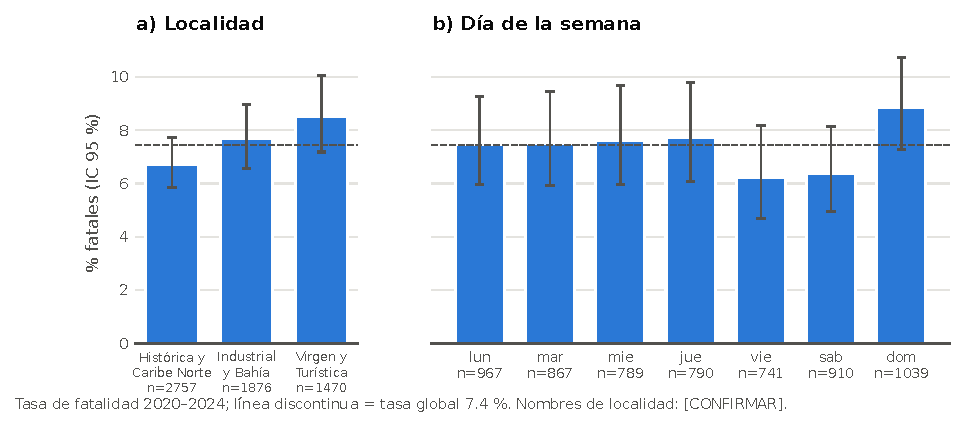
\includegraphics[width=0.8\textwidth]{figuras/fig4_tasa_por_localidad_y_dia.pdf}
\caption{Tasa de fatalidad por localidad y por día de la semana (2020--2024), con IC 95\,\%.}\label{fig:loc}
\end{figure*}

\begin{figure}[t]
\centering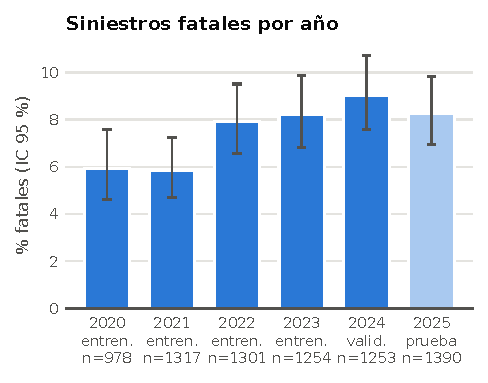
\includegraphics[width=0.85\columnwidth]{figuras/fig1_tasa_por_anio.pdf}
\caption{Tasa de fatalidad por año con IC 95\,\% (Wilson). La prevalencia crece en el periodo; 2025 es la prueba.}\label{fig:anio}
\end{figure}
\begin{figure}[t]
\centering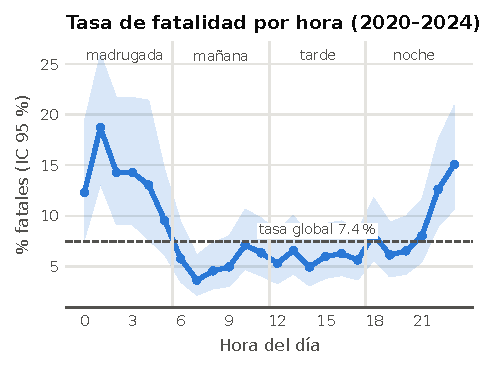
\includegraphics[width=0.85\columnwidth]{figuras/fig2_tasa_por_hora.pdf}
\caption{Tasa de fatalidad por hora (2020--2024): fuerte y no lineal, con máximo en la madrugada.}\label{fig:hora}
\end{figure}
\begin{figure*}[t]
\centering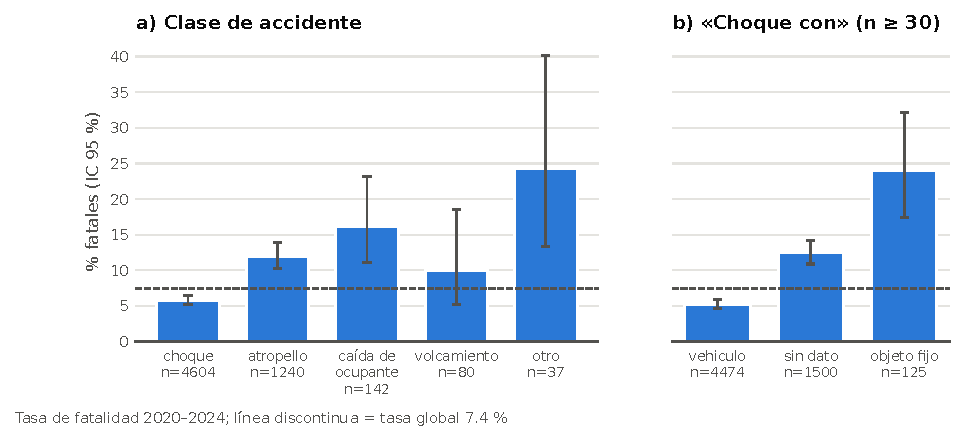
\includegraphics[width=0.8\textwidth]{figuras/fig3_tasa_por_clase_y_choque.pdf}
\caption{Tasa de fatalidad por clase de accidente y por «choque con» (2020--2024), con IC 95\,\%.}\label{fig:clase}
\end{figure*}

% =====================================================================================================================
\section{Método}
\textbf{Línea base.} Clasificador mayoritario y regresión logística sin ajuste ($C=1$, pesos de clase balanceados, umbral 0,5),
con imputación por mediana, estandarización y codificación \emph{one-hot} (categorías con menos de 20 casos agrupadas).

\textbf{Modelos propuestos.} (a) Regresión logística ajustada ($C\in\{0{,}01;0{,}1;1;10\}$), para separar el efecto del ajuste del
de la familia de modelo. (b) \emph{Random forest} \cite{breiman2001rf} de 300 árboles, con rejilla sobre el tamaño mínimo de hoja
$\{5,20,50\}$, la fracción de variables por división $\{\sqrt{p},\,0{,}3\}$ y el peso de clases (balanceado o no). (c)
\emph{HistGradientBoosting} \cite{ke2017lightgbm,pedregosa2011sklearn} con categóricas nativas, parada temprana, tasa de
aprendizaje $\{0{,}03;0{,}1\}$, hojas $\{8,31\}$, mínimo por hoja $\{20,80\}$ y peso de clases. Elegimos árboles porque la
exploración mostró relaciones no lineales (hora) e interacciones (clase $\times$ franja) que la regresión lineal no captura
\cite{russell2020aima}.

\textbf{Protocolo.} Cada una de las \CifraNConfig{} configuraciones se evaluó con origen móvil
\cite{tashman2000outofsample} (2020--21$\to$2022, 2020--22$\to$2023, 2020--23$\to$2024) y cinco semillas (42--46); dentro de cada
familia se eligió la configuración con mayor PR-AUC medio en los tres pliegues, y entre familias, la de mayor PR-AUC medio. El
umbral se fijó en validación 2024 con la regla de recall $\geq 0{,}60$. Además, se hizo una ablación de conjuntos de variables:
\texttt{contexto} (cuándo y dónde), \texttt{reporte} (principal) e \texttt{hipotesis} (más la hipótesis causal del agente de
tránsito, que puede formarse después del hecho y por eso solo se usa como análisis). La Fig.~\ref{fig:arq} resume la arquitectura.

\textbf{Alternativas consideradas.} Redes neuronales (descartadas: \CifraNTrain{} ejemplos de entrenamiento y variables tabulares
de baja dimensión), sobremuestreo sintético (no usado: los pesos de clase resuelven el desbalance sin crear registros artificiales)
y validación cruzada aleatoria (descartada por la deriva temporal).

\begin{figure}[t]
\centering
\resizebox{\columnwidth}{!}{%
\begin{tikzpicture}[node distance=3mm and 3mm, every node/.style={font=\scriptsize, align=center},
  caja/.style={draw, rounded corners=2pt, minimum height=6mm, inner sep=2pt, fill=blue!5},
  datos/.style={draw, minimum height=6mm, inner sep=2pt, fill=orange!10}, flecha/.style={-{Stealth[length=1.6mm]}}]
\node[datos] (raw) {CSV DATT\\(CC-BY, SHA-256)};
\node[caja, right=of raw] (pre) {Limpieza, etiqueta,\\dedup., v3.1};
\node[datos, right=of pre] (part) {Partición\\temporal};
\node[caja, below=5mm of raw] (mov) {Rejilla + origen\\móvil + 5 semillas};
\node[caja, right=of mov] (sel) {Elección por\\PR-AUC; umbral\\(recall $\geq$ 0,6)};
\node[caja, right=of sel] (test) {Prueba 2025\\(una vez)};
\node[caja, below=7mm of mov] (err) {Errores y\\deriva};
\node[caja, right=of err] (resp) {Subgrupos e\\IA responsable};
\node[caja, right=of resp] (app) {Prototipo\\Streamlit};
\draw[flecha] (raw) -- (pre); \draw[flecha] (pre) -- (part); \draw[flecha] (part.south) |- ++(0,-1.5mm) -| (mov.north);
\draw[flecha] (mov) -- (sel); \draw[flecha] (sel) -- (test);
\draw[flecha] (test.south) |- ++(0,-3.5mm) -| (err.north); \draw[flecha] (err) -- (resp); \draw[flecha] (resp) -- (app);
\end{tikzpicture}}
\caption{Arquitectura del sistema. Cada etapa es un script de \texttt{src/} y escribe sus resultados en \texttt{experiments/}.}\label{fig:arq}
\end{figure}

% =====================================================================================================================
\section{Experimentos y resultados}
\textbf{Configuración.} Python 3.13, scikit-learn 1.9.1, semilla 42; la búsqueda completa tarda \CifraDuracionBusqueda{}\,s.
Métricas primarias: PR-AUC (azar = prevalencia, \CifraBaseAzar{} en 2024) y F1 de la clase fatal; secundarias: ROC-AUC, precisión,
recall, matriz de confusión y recall por subgrupo. La exactitud no se usa: predecir siempre «no fatal» da \CifraBaseAcc{}.
Criterios de éxito (declarados antes de entrenar): (1) PR-AUC al menos 0,05 mayor que la línea base; (2) ROC-AUC $\geq 0{,}70$;
(3) precisión $\geq 0{,}20$ con recall $\geq 0{,}60$; (4) ningún subgrupo elegible con recall más de 0,15 por debajo del global.

\textbf{Validación.} La Tabla~\ref{tab:comp} compara los modelos. El \emph{random forest} (hoja mínima \CifraRFHojas{},
\texttt{max\_features}=\CifraRFMaxFeat{}, sin pesos de clase) fue elegido por tener el mayor PR-AUC medio en los tres pliegues
(\CifraValPRMovil{}); en 2024 obtuvo \CifraValPR{}\,$\pm$\,\CifraValPRsd{}, apenas \CifraValDifPR{} sobre la línea base, y ROC-AUC
\CifraValROC{}. Su umbral, \CifraUmbral{}, da en validación precisión \CifraValPrec{} y recall \CifraValRec{}. La ablación
(Tabla~\ref{tab:abl}) muestra que el informe añade señal sobre el contexto (\CifraAblContexto{}$\to$\CifraAblReporte{}) y que la
hipótesis del agente añade bastante más (\CifraAblHipotesis{}; ROC-AUC \CifraAblHipotesisROC{}), lo que sugiere que el techo
proviene de la información disponible y no de la capacidad del modelo.

\begin{table}[t]
\caption{Validación (2024, variables \texttt{reporte}; media $\pm$ desv. de 5 semillas; «mov.» = media de los 3 pliegues de origen móvil)}\label{tab:comp}
\centering\resizebox{\columnwidth}{!}{\begin{tabular}{@{}lcccc@{}}
\toprule
Modelo & PR-AUC & PR-AUC & ROC-AUC & Prec. \\
 & mov. & 2024 & 2024 & rec.$\geq$0,6 \\
\midrule
{Línea base (RL, $C{=}1$)} & 0,166 & 0,220 & 0,666 & 0,152 \\
{RL ajustada} & 0,172 & 0,226 & 0,683 & 0,146 \\
\textbf{Random forest} & 0,180 & 0,224 $\pm$ 0,004 & 0,699 $\pm$ 0,006 & 0,166 $\pm$ 0,009 \\
{HistGradientBoosting} & 0,168 & 0,194 $\pm$ 0,019 & 0,658 $\pm$ 0,009 & 0,138 $\pm$ 0,005 \\
\bottomrule
\end{tabular}
}
\end{table}
\begin{table}[t]
\caption{Ablación: PR-AUC en validación 2024 por conjunto de variables}\label{tab:abl}
\centering\resizebox{0.9\columnwidth}{!}{\begin{tabular}{@{}lccc@{}}
\toprule
Modelo & \texttt{contexto} & \texttt{reporte} & \texttt{hipotesis} \\
\midrule
Línea base (RL, $C{=}1$) & 0,166 & 0,220 & 0,272 \\
Random forest & 0,176 & 0,224 & 0,273 \\
HistGradientBoosting & 0,155 & 0,194 & 0,243 \\
\bottomrule
\end{tabular}
}
\end{table}

\textbf{Prueba (2025, evaluada una vez desde el commit \texttt{\CifraCommitFinal}).} Entrenados con 2020--2024, el \emph{random
forest} supera a la línea base en PR-AUC (\CifraTestPR{} frente a \CifraTestBasePR{}, diferencia \CifraTestDifPR{}) y alcanza ROC-AUC
\CifraTestROC{} \CifraTestROCic{} (Tabla~\ref{tab:prueba}). Pero con el umbral de validación alerta en el \CifraTestAlerta{} de los
casos y detecta \CifraTestTP{} de \CifraFatTest{} fatales (recall \CifraTestRec{}), con precisión \CifraTestPrec{}. La
Tabla~\ref{tab:crit} resume los criterios: se cumple solo el 2 en prueba.

\begin{table*}[t]
\caption{Prueba 2025 ($n=\CifraNTest$, \CifraFatTest{} fatales). Debajo de cada valor, IC 95\,\% por \emph{bootstrap} (1.000 remuestreos)}\label{tab:prueba}
\centering\small\begin{tabular}{@{}lcccccc@{}}
\toprule
Modelo & Umbral & PR-AUC & ROC-AUC & Prec. & Recall & F1 \\
\midrule
Random forest & 0,109 & 0,223 & 0,712 & 0,157 & 0,470 & 0,236 \\
 & & [0,17; 0,30] & [0,67; 0,76] & [0,12; 0,20] & [0,38; 0,56] & \\
\midrule
Línea base & 0,500 & 0,154 & 0,689 & 0,137 & 0,574 & 0,221 \\
 & & [0,12; 0,20] & [0,65; 0,73] & [0,11; 0,17] & [0,49; 0,66] & \\
\midrule
Línea base & 0,552 & 0,154 & 0,689 & 0,152 & 0,504 & 0,234 \\
 & & [0,12; 0,20] & [0,65; 0,73] & [0,12; 0,19] & [0,42; 0,59] & \\
\bottomrule
\end{tabular}

\end{table*}
\begin{table}[t]
\caption{Criterios de éxito predeclarados}\label{tab:crit}
\centering\resizebox{\columnwidth}{!}{\begin{tabular}{@{}lcc@{}}
\toprule
Criterio & Valor & Cumple \\
\midrule
1. PR-AUC $\geq$ base + 0,05 (val.) & 0,224 & No \\
2. ROC-AUC $\geq$ 0,70 (val.) & 0,699 & No \\
2. ROC-AUC $\geq$ 0,70 (prueba) & 0,712 & Sí \\
3. Prec. $\geq$ 0,20 con rec. $\geq$ 0,60 & P=0,157, R=0,470 & No \\
4. Brecha de recall $\leq$ 0,15 & Tarde: 0,352 & No \\
\bottomrule
\end{tabular}
}
\end{table}

\textbf{Deriva del umbral.} El recall cayó de \CifraValRec{} a \CifraTestRec{} porque las probabilidades bajaron en 2025 (media
\CifraProbaVal{}$\to$\CifraProbaTest{}; alertas \CifraAlertaVal{}$\to$\CifraAlertaTest{}), en un año en que la tasa real de
atropellos fue \CifraAtropelloTest{} (\CifraAtropelloVal{} en 2024) y la de la tarde \CifraTardeTest{} (\CifraTardeVal{}). Un
umbral de probabilidad absoluto no se trasladó bien entre años.

\textbf{Análisis de errores.} Clasificamos con reglas explícitas los \CifraNFN{} falsos negativos y \CifraNFP{} falsos positivos
(Tabla~\ref{tab:err}); la tabla detallada de los 20 errores de mayor confianza, con variables e hipótesis, está en
\texttt{experiments/analisis\_errores.csv}. \CifraFNChoqueVeh{} de los \CifraNFN{} falsos negativos son choques entre vehículos:
su informe inicial es casi idéntico al de miles de choques con heridos, y lo que los hace fatales (tipo de vehículo, velocidad,
casco, edad) no está en los datos \pend{CONFIRMAR hipótesis}. Los falsos positivos se concentran en atropellos (\CifraFPAtropello{})
y en choques nocturnos o contra objeto fijo: perfiles de alto riesgo cuyo desenlace no fue fatal (Tabla~\ref{tab:ej}). Por
permutación en validación, las variables más útiles son \CifraImpUno{} (\CifraImpUnoVal{} de PR-AUC), \CifraImpDos{}
(\CifraImpDosVal{}) y \CifraImpTres{} (\CifraImpTresVal{}).

\begin{table}[t]
\caption{Errores en prueba por categoría}\label{tab:err}
\centering\resizebox{\columnwidth}{!}{\begin{tabular}{@{}llr@{}}
\toprule
Cód. & Categoría (regla en \texttt{src/errors.py}) & $n$ \\
\midrule
FN1 & Choque entre vehículos de día (mañana/tarde) & 17 \\
FN2 & Choque entre vehículos de noche/madrugada & 30 \\
FN3 & Atropello o caída de ocupante con baja probabilidad & 13 \\
FN4 & Otros & 1 \\
FP1 & Choque contra objeto fijo & 55 \\
FP2 & Atropello & 144 \\
FP3 & Choque vehicular de noche/madrugada & 37 \\
FP4 & Otros (volcamiento, caída de ocupante, choque diurno) & 53 \\
\bottomrule
\end{tabular}
}
\end{table}
\begin{table}[t]
\caption{Ejemplos de errores de mayor confianza (3 FN y 3 FP)}\label{tab:ej}
\centering\resizebox{\columnwidth}{!}{\begin{tabular}{@{}rcccl@{}}
\toprule
IPAT & Tipo & Prob. & Cat. & clase; choque con; franja \\
\midrule
1340069 & FN & 0,016 & FN1 & choque; vehiculo; tarde \\
1339287 & FN & 0,016 & FN1 & choque; vehiculo; tarde \\
1339719 & FN & 0,024 & FN2 & choque; vehiculo; noche \\
1339542 & FP & 0,368 & FP1 & choque; objeto fijo; madrugada \\
1339187 & FP & 0,355 & FP3 & choque; vehiculo; noche \\
1340129 & FP & 0,340 & FP3 & choque; vehiculo; madrugada \\
\bottomrule
\end{tabular}
}
\end{table}

% =====================================================================================================================
\section{IA responsable y limitaciones}
\textbf{Equidad por franja y localidad (medida).} El recall por subgrupo (Fig.~\ref{fig:sub}) es \CifraTestRecMadrugada{} en la
madrugada, \CifraTestRecManana{} en la mañana, \CifraTestRecNoche{} en la noche y \CifraTestTardeRec{} \CifraTestTardeic{} en la
tarde, que incumple el criterio 4 con solo \CifraTestTardeFat{} fatales (brecha \CifraTestBrechaTarde{}, frente a
\CifraTestBrechaTardeBase{} de la línea base). Por localidad, el recall es \CifraTestRecLocUno{} \CifraTestRecLocUnoic{},
\CifraTestRecLocDos{} \CifraTestRecLocDosic{} y \CifraTestRecLocTres{} \CifraTestRecLocTresic{} en las localidades 1, 2 y 3:
ninguna incumple el criterio, aunque la 2 queda cerca. En validación el subgrupo que fallaba era la \CifraValPeorSubgrupo{}
(\CifraValPeorRecall{}): con tan pocos casos no se distingue un sesgo estable del ruido, pero sí que el modelo detecta peor los
fatales diurnos. \emph{Mitigación:} reportar siempre el recall por franja con su intervalo y advertirlo en el prototipo; como
trabajo futuro, umbrales por franja elegidos en validación.

\textbf{Estigmatización de barrios (medida).} En Mamonal el modelo alerta en el \CifraMamonalAlerta{} de los siniestros
(\CifraMamonalVeces{} veces la tasa global de alerta) con una tasa real de \CifraMamonalReal{}. La ubicación pesa en el modelo y
refleja vías y tráfico, no a los habitantes. \emph{Mitigación:} el prototipo no muestra mapas ni rankings de barrios y la alerta
es por siniestro, nunca para asignar vigilancia.

\textbf{Alcance y uso.} El modelo no decide si hay víctimas; solo estima la gravedad cuando ya se sabe que las hay. Con precisión
\CifraTestPrec{}, la mayoría de las alertas son falsas: es una herramienta de apoyo y nunca justifica reducir la atención de un caso.

\textbf{Calidad de datos.} La columna \texttt{muertos} es inconsistente en 2025; puede haber sub-registro de muertes posteriores al
informe \pend{VERIFICAR con el DATT cuándo se actualiza la gravedad}; los códigos de localidad se tradujeron con evidencia indirecta
\pend{CONFIRMAR}. \textbf{Limitaciones.} Faltan variables clave (vehículo, víctima, velocidad); la deriva temporal afecta al umbral;
los subgrupos tienen pocos fatales; el conjunto \texttt{hipotesis} no se usa por su posible información posterior al hecho.

\begin{figure}[t]
\centering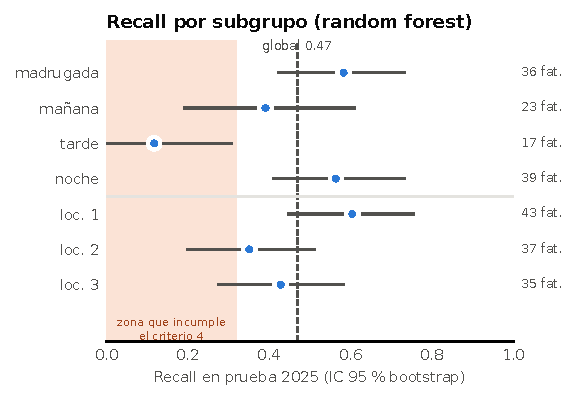
\includegraphics[width=0.9\columnwidth]{figuras/fig5_recall_subgrupos.pdf}
\caption{Recall por subgrupo en prueba con IC 95\,\%. La zona sombreada incumple el criterio 4 (más de 0,15 bajo el global).}\label{fig:sub}
\end{figure}

% =====================================================================================================================
\section{Conclusiones y trabajo futuro}
\textbf{Respuesta a la pregunta.} Sí hay señal: con solo el informe inicial, el \emph{random forest} ordena los siniestros mejor que
el azar (PR-AUC \CifraTestPR{} frente a una prevalencia de \CifraPctTest{}) y que la línea base en la prueba, con ROC-AUC
\CifraTestROC{}. Pero no es suficiente para el uso previsto: no supera a la línea base por el margen fijado en validación
(+\CifraValDifPR{} frente a +0,05), su precisión en el punto de operación es \CifraTestPrec{} y su recall cae en la tarde. Las
diferencias por franja horaria son mayores que por localidad, tanto en la tasa real de fatalidad como en el desempeño del modelo. Consideramos este resultado negativo como el hallazgo principal: el cuello
de botella es la información del informe inicial, como sugiere la ablación con la hipótesis del agente.

\textbf{Trabajo futuro.} (1) Incorporar variables del vehículo y la víctima si el DATT las publica, en particular la participación
de motocicletas; (2) recalibrar el umbral cada año o usar umbrales por franja; (3) consultar al DATT la inconsistencia de 2025 y el
diccionario de localidades; (4) evaluar el costo de los errores como en \cite{iranitalab2017comparison}.

% =====================================================================================================================
\section{Contribuciones y declaración de uso de IA generativa}
\textbf{Contribuciones.} \pend{COMPLETAR POR EL EQUIPO: qué hizo cada integrante (datos, modelos, análisis, prototipo, informe,
sustentación).}

\textbf{Uso de IA generativa.} Se usaron Claude (chat) y Claude Code para proponer temas, escribir código del pipeline, pruebas,
análisis y un borrador de este informe; cada uso está registrado en \texttt{docs/bitacora\_ia.md} con lo aceptado, lo descartado y
cómo se verificó. \pend{COMPLETAR POR EL EQUIPO: herramientas y alcance exactos.}

\textbf{Reflexión (borrador \pend{COMPLETAR POR EL EQUIPO}).} La IA propuso cosas incorrectas varias veces y la verificación
contra los datos reales lo reveló. Diseñó la etiqueta con la clase «Solo daños materiales» sin haber visto los datos, y el
preprocesamiento mostró que esa clase no existe. Sugirió redefinir la etiqueta con \texttt{muertos}, columna que resultó errónea en
2025. En la fase final predijo que, al reentrenar con 2020--2024, el umbral de validación daría \emph{más} alertas y \emph{más}
recall en la prueba; ocurrió lo contrario, y lo detectamos al comparar las distribuciones de probabilidad de ambos años. También
detectó un error real (la variable \texttt{tipo\_via} constante), pero solo porque se le pidió verificar los datos antes de modelar.
Lección: tratar cada afirmación de la IA como una hipótesis y contrastarla con los datos o con una fuente primaria.
\pend{COMPLETAR POR EL EQUIPO: caso propio, en primera persona, y qué cambiarían.}

% =====================================================================================================================
\bibliographystyle{IEEEtran}
\bibliography{referencias}

\end{document}
